% Name: Shengfeng Li
% Project: PA-2 (Writing)
% Instructor: Feng Chen
% Class: cs7103-au18
% LogonID: cs710305
% This is "sig-alternate.tex" V2.0 May 2012
% This file should be compiled with V2.5 of "sig-alternate.cls" May 2012
%
% This example file demonstrates the use of the 'sig-alternate.cls'
% V2.5 LaTeX2e document class file. It is for those submitting
% articles to ACM Conference Proceedings WHO DO NOT WISH TO
% STRICTLY ADHERE TO THE SIGS (PUBS-BOARD-ENDORSED) STYLE.
% The 'sig-alternate.cls' file will produce a similar-looking,
% albeit, 'tighter' paper resulting in, invariably, fewer pages.
%
% ----------------------------------------------------------------------------------------------------------------
% This .tex file (and associated .cls V2.5) produces:
%       1) The Permission Statement
%       2) The Conference (location) Info information
%       3) The Copyright Line with ACM data
%       4) NO page numbers
%
% as against the acm_proc_article-sp.cls file which
% DOES NOT produce 1) thru' 3) above.
%
% Using 'sig-alternate.cls' you have control, however, from within
% the source .tex file, over both the CopyrightYear
% (defaulted to 200X) and the ACM Copyright Data
% (defaulted to X-XXXXX-XX-X/XX/XX).
% e.g.
% \CopyrightYear{2007} will cause 2007 to appear in the copyright line.
% \crdata{0-12345-67-8/90/12} will cause 0-12345-67-8/90/12 to appear in the copyright line.
%
% ---------------------------------------------------------------------------------------------------------------
% This .tex source is an example which *does* use
% the .bib file (from which the .bbl file % is produced).
% REMEMBER HOWEVER: After having produced the .bbl file,
% and prior to final submission, you *NEED* to 'insert'
% your .bbl file into your source .tex file so as to provide
% ONE 'self-contained' source file.
%
% ================= IF YOU HAVE QUESTIONS =======================
% Questions regarding the SIGS styles, SIGS policies and
% procedures, Conferences etc. should be sent to
% Adrienne Griscti (griscti@acm.org)
%
% Technical questions _only_ to
% Gerald Murray (murray@hq.acm.org)
% ===============================================================
%
% For tracking purposes - this is V2.0 - May 2012
\documentclass{sig-alternate}
\usepackage{comment}
\usepackage{tabularx}
\newcolumntype{C}{>{\centering\arraybackslash}X}
\renewcommand\tabularxcolumn[1]{>{\centering}m{#1}}
\usepackage{array}
\usepackage{multirow}

\begin{document}
%
% --- Author Metadata here ---
\conferenceinfo{SOSP}{'97 El Paso, Texas USA}
%\CopyrightYear{2007} % Allows default copyright year (20XX) to be over-ridden - IF NEED BE.
%\crdata{0-12345-67-8/90/01}  % Allows default copyright data (0-89791-88-6/97/05) to be over-ridden - IF NEED BE.
% --- End of Author Metadata ---

\title{Docker is Not a Virtual Machine}
%\subtitle{[Extended Abstract]
%\titlenote{A full version of this paper is available as
%\textit{Author's Guide to Preparing ACM SIG Proceedings Using
%\LaTeX$2_\epsilon$\ and BibTeX} at
%\texttt{www.acm.org/eaddress.htm}}}
%
% You need the command \numberofauthors to handle the 'placement
% and alignment' of the authors beneath the title.
%
% For aesthetic reasons, we recommend 'three authors at a time'
% i.e. three 'name/affiliation blocks' be placed beneath the title.
%
% NOTE: You are NOT restricted in how many 'rows' of
% "name/affiliations" may appear. We just ask that you restrict
% the number of 'columns' to three.
%
% Because of the available 'opening page real-estate'
% we ask you to refrain from putting more than six authors
% (two rows with three columns) beneath the article title.
% More than six makes the first-page appear very cluttered indeed.
%
% Use the \alignauthor commands to handle the names
% and affiliations for an 'aesthetic maximum' of six authors.
% Add names, affiliations, addresses for
% the seventh etc. author(s) as the argument for the
% \additionalauthors command.
% These 'additional authors' will be output/set for you
% without further effort on your part as the last section in
% the body of your article BEFORE References or any Appendices.

\numberofauthors{1} %  in this sample file, there are a *total*
% of EIGHT authors. SIX appear on the 'first-page' (for formatting
% reasons) and the remaining two appear in the \additionalauthors section.
%
\author{
% You can go ahead and credit any number of authors here,
% e.g. one 'row of three' or two rows (consisting of one row of three
% and a second row of one, two or three).
%
% The command \alignauthor (no curly braces needed) should
% precede each author name, affiliation/snail-mail address and
% e-mail address. Additionally, tag each line of
% affiliation/address with \affaddr, and tag the
% e-mail address with \email.
%
% 1st. author
\alignauthor
Shengfeng Li\\
       \affaddr{Computer Science Department}\\
       \affaddr{Louisiana State University}\\
       \affaddr{Baton Rouge, Louisiana 70803, USA}\\
       \email{sli49@lsu.edu}
% 2nd. author
%\alignauthor
%G.K.M. Tobin\titlenote{The secretary disavows
%any knowledge of this author's actions.}\\
%       \affaddr{Institute for Clarity in Documentation}\\
%       \affaddr{P.O. Box 1212}\\
%       \affaddr{Dublin, Ohio 43017-6221}\\
%       \email{webmaster@marysville-ohio.com}
}
% There's nothing stopping you putting the seventh, eighth, etc.
% author on the opening page (as the 'third row') but we ask,
% for aesthetic reasons that you place these 'additional authors'
% in the \additional authors block, viz.
%\additionalauthors{Additional authors: John Smith (The Th{\o}rv{\"a}ld Group,
%email: {\texttt{jsmith@affiliation.org}}) and Julius P.~Kumquat
%(The Kumquat Consortium, email: {\texttt{jpkumquat@consortium.net}}).}
\date{30 July 1999}
% Just remember to make sure that the TOTAL number of authors
% is the number that will appear on the first page PLUS the
% number that will appear in the \additionalauthors section.

\maketitle
\begin{abstract}
Virtual Machine was defined as an efficient, isolated duplicate of a real computer machine. It dates to the 1960s\cite{wiki:vm} and still widely be used in operating systems. Docker, on the other hand, is also a computer program that provides an environment that can run other applications on top of the kernel in an isolated way and it is still a very young program debuted in 2013\cite{wiki:docker}. Many people might think that docker is some sort of \textit{lightweight} or \textit{trimmed down} Virtual Machine but it's actually not. Though Virtual Machine and docker both run on the top of any operating system, they have very different architectures. Both of them have their own usage scenarios. 
\end{abstract}


% A category with the (minimum) three required fields
%\category{H.4}{Information Systems Applications}{Miscellaneous}
%A category including the fourth, optional field follows...
%\category{D.2.8}{Software Engineering}{Metrics}[complexity measures, performance measures]

%\terms{Theory}

%\keywords{ACM proceedings, \LaTeX, text tagging}


\section{Introduction}
This paper tries to illustrate the architecture of Virtual Machine and the docker. And by comparing the difference between them, it helps us obtain a better perspective about which technology fits your scenario better. Virtual Machine technology has been developing for more than 50 years. It is universally known and is still widely used. Docker, on the other way, is very young compared to Virtual Machine and is becoming more and more popular these days as it can avoid the \textit{overhead} of resource utilization.

A virtual machine emulates a physical computing environment, but requests for CPU, memory, hard disk, network and other hardware resources. Those requests are managed by a virtualization layer which translates these requests to the underlying physical hardware. Virtual machines are powered by hypervisors which is a software that can provide isolation for virtual machines running on top of the physical host. In another word, you can several virtual machines running simultaneously on a infrastructure without interfering with each other. Many cloud infrastructure providers such virtualization such as Google Compute Engine, Microsoft Azure and Amazon EC2. However, since all the virtual machines need to require their own hardware resource, resource overhead is involved. 

Docker is a modern open source platform. The goal of docker is to make development, shipment, and deployment easier for developers. When Docker emerged in 2013, container exploded in popularity. Docker is a very new software. However, the technology docker originally used was Linux Containers(LXC)\footnote{LXC is the well known set of tools, templates, library and language bindings. It's pretty low level, very flexible and covers just about every containment feature supported by the upstream kernel.}. LXC was the first, most complete implementation of Linux container manager and it was implemented in 2008. LXC can run on a single Linux kernel without requiring any patches. And in the later year, docker replaced LXC container manager with its own library, libcontainer(runC)\footnote{runC is a CLI tool for spawning and running containers according to the OCI specification}. A container is an image generated by the docker which has all the supporting dependencies packaged into a standard form. Containers also run on top of the kernel but share the hardware resource with the kernel. This architecture makes container much lighter than the virtual machine, hence extremely improve the performance. And the containers keep running in an isolated way as well.

This paper is a review of the technology of Virtual Machine and Docker and will compare the performance between those two technologies. The article is organized as follow. Section 2 will introduce the technology of virtual machine and talk about some disadvantages of Virtual Machine. Section 3 will introduce the technology of docker and the advantages and disadvantages of Docker container. Section 4 will focus on the comparison between docker and virtual machine. Section 5 will be a short summary, following with a conclusion. 

\section{Virtual Machine}
Virtual Machine begins with some type of infrastructure which could be your laptop, a dedicated server running in a data center or a virtual private server that you're using in the cloud such as Digital Ocean, Google Compute Engine, Microsoft Azure and Amazon EC2 etc. On top of the infrastructure runs an operating system that could be Mac OS, Windows or some distribution of Linux. When we talking about VMs(Virtual machines), the operating system is commonly labeled as the host. Above the host operating system, we have a thing called hypervisor. A hypervisor is a software which provides isolation for virtual machines running on top of host operating system. We can think of Virtual Machine as a self-contained computer packed into a single file but something needs to be able to run that file. That's where a hypervisor comes into play. There are two types of hypervisors. The first type of hypervisors directly links to the infrastructure such as HyperKit(OSX), Hyper-V(Win) and KVM(Linux). Another one runs an application on the host operating system such as VirtualBox and VMWare. Usually, hypervisors belong to the first type are more efficient because they can bypass the host operating system and directly interact with the hardware of the server. The next layer above the hypervisor is the guest operating systems\footnote{VM is called as the guest while the environment it runs on is called the host}. We can run as many guest OS as possible as long as the infrastructure can afford the hardware resource requirement in total isolation. Those guest operating systems are all controlled by the hypervisor and are not required to be the same. We could run Windows, Mac OS, distribution Linux, and other supported OS.  On top of the OS, there are applications and libraries. The Figure \ref{fig:vma} shows the architecture of the virtual machine. 

\begin{figure}[ht]
\centering
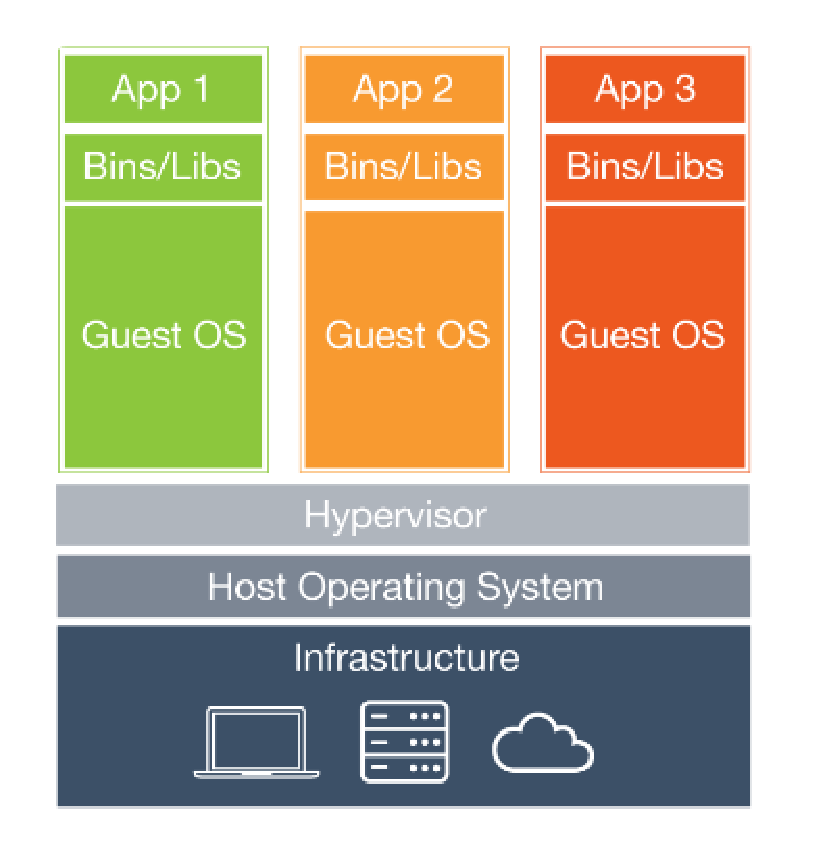
\psfig{file=VM_architecture.eps, height=2in, width=2in,}
\caption{Virtual Machine Architecture}
\label{fig:vma}
\vskip -6pt
\end{figure}

\subsection{Disadvantage of Virtual Machine}
Each guest OS requires its own requirement of hardware resources. Assume each guest OS require 1GB disk space, then the total disk space required would be 1GB $\times$ 3. Not to mention other requirements such as CPU, memory, and network. Whenever an instance starts within the virtual environment, all the resources that have been assigned to it start being used. So if you assign four gigabytes of RAM to a virtual server as soon as that virtual server has started, four gigabytes of RAM from the hardware will automatically be assigned to that virtual server. If you have three servers that boot up with four gigabytes of RAM, 4GB $\times$ 3 will be allocated to those servers whether or not they actually need it. Each one of those servers may only need one gigabyte RAM currently and other idle RAM can't be given somewhere else. Every single instance of an operating system has to have these over-allocated resources allocated to it and  This results in a lot of resources wasted. Another issue is that the virtual machine emulating an entire server which means you have to run the whole boot up process. Suppose you create a virtual server that only does DNS, when you do some configuration, you have to reboot the entire computer and going through the whole boot process which takes a lot of time. 

\section{Docker Containers}
Firstly, the docker containers also need the infrastructure. The second level is the host operating system. Then we have a layer called docker daemon. Docker daemon is a service that runs in the background on our host OS and manages everything required to run and interact with docker containers. After that, we have binaries and libraries just like the virtual machines but instead of running on a guest OS, they get built into special packages called docker images. The docker daemon runs those images. The applications would end up residing in its own docker image and will be managed independently by the docker daemon. Typically, each application and its library dependencies get packed into the same docker image. Each application is still isolated. In the docker scenario, we don't need to run any type of hypervisor or virtual machine. Instead, the docker daemon communicates directly with the host operating system and knows how to ration the resources for the running docker containers. It's also an expert and ensuring each container is isolated from both the host OS and other containers. There is also no virtualization needed with docker since it runs directly on the host OS. Figure \ref{fig:da} shows the architecture of the docker. 

\begin{figure}[ht]
\centering
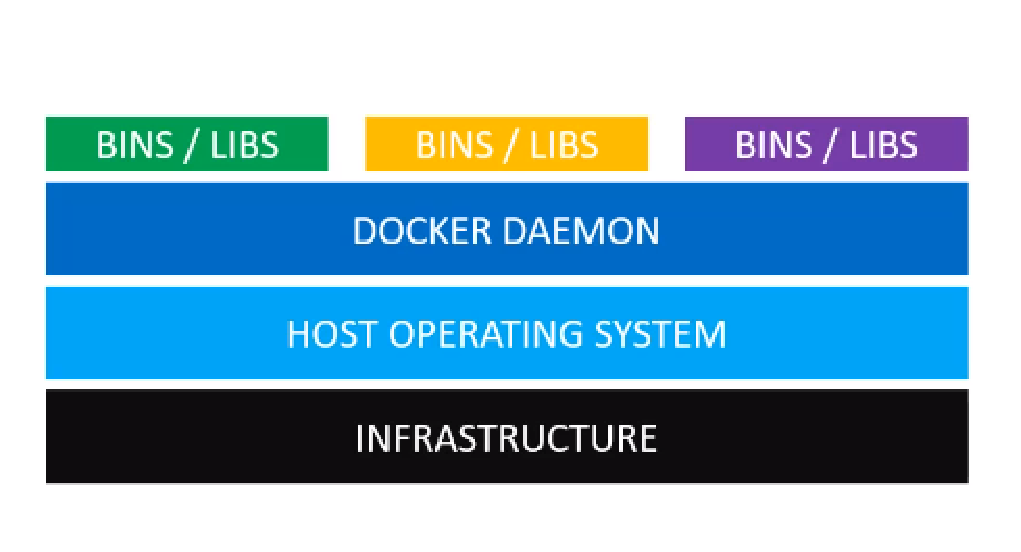
\psfig{file=docker_architecture.eps, height=2in, width=2in,}
\caption{Docker Architecture}
\label{fig:da}
\vskip -6pt
\end{figure}

\subsection{Advantage of Docker(LXC)}
LXC, also known as Linux container, is created for the services the virtual servers will provide. The underlying hardware resources and kernel is shared from all the containers. You can have one container that is equivalent of a LAMP\footnote{LAMP is an open source Web development platform that uses Linux as the operating system, Apache as the Web server, MySQL as the rational database management system and PHP/Perl/Python as the object-oriented scripting language.} server which has all the required software installed, the configuration files and IP address etc. But the container doesn't have the kernel and the RAM directly associated with it. The kernel and the RAM and some other resources and on the lower level. You can also have a DNS or a DHCP or a file server container at the same time besides the LAMP container. Those containers share the underlying RAM, hard drive, CPU and the kernel. RAM still be controlled by the single host kernel who is expert. It's like running services on any kind of server. You don't need to worry about RAM or hard drive allocation. Furthermore, When one of the servers needs to be restart, you don't need to have the boot process like the virtual machine has. Also, the containers are completely segregated. They have their own IP addresses. They interact with the rest of the network such as the host and other containers just like they are individual servers but using the same kernel. 

\subsection{Disadvantage of Docker Container}
Even though there are some improvements of container comparing to Virtual Machine, there are some drawbacks of Docker Container too. 
\begin{itemize}
\item As containers share the kernel with the host, you cannot have a windows container running on a Linux kernel.
\item Since containers need to be the same with the host kernel, you cannot have multiple different containers running at the same time. 
\item The container is more like a service, it does not provide you with the complete virtualization.
\item Docker is still young. It requires some new built-in features to support containers such as LXC or runC. Many old machines will not able to use Docker.
\item Thought docker supports cross-platform, the containers might not work the same in different systems and even different distributions. In Linux, the kernels in different distribution, such as Ubuntu, Fedora and CentOS etc, are not consistent.
\item Security issues need to be evaluated. The kernel is shared among containers. Containers could be malicious. 
\end{itemize}

\section{Container vs. Virtual Machines}

\begin{figure}[htb]
\centering
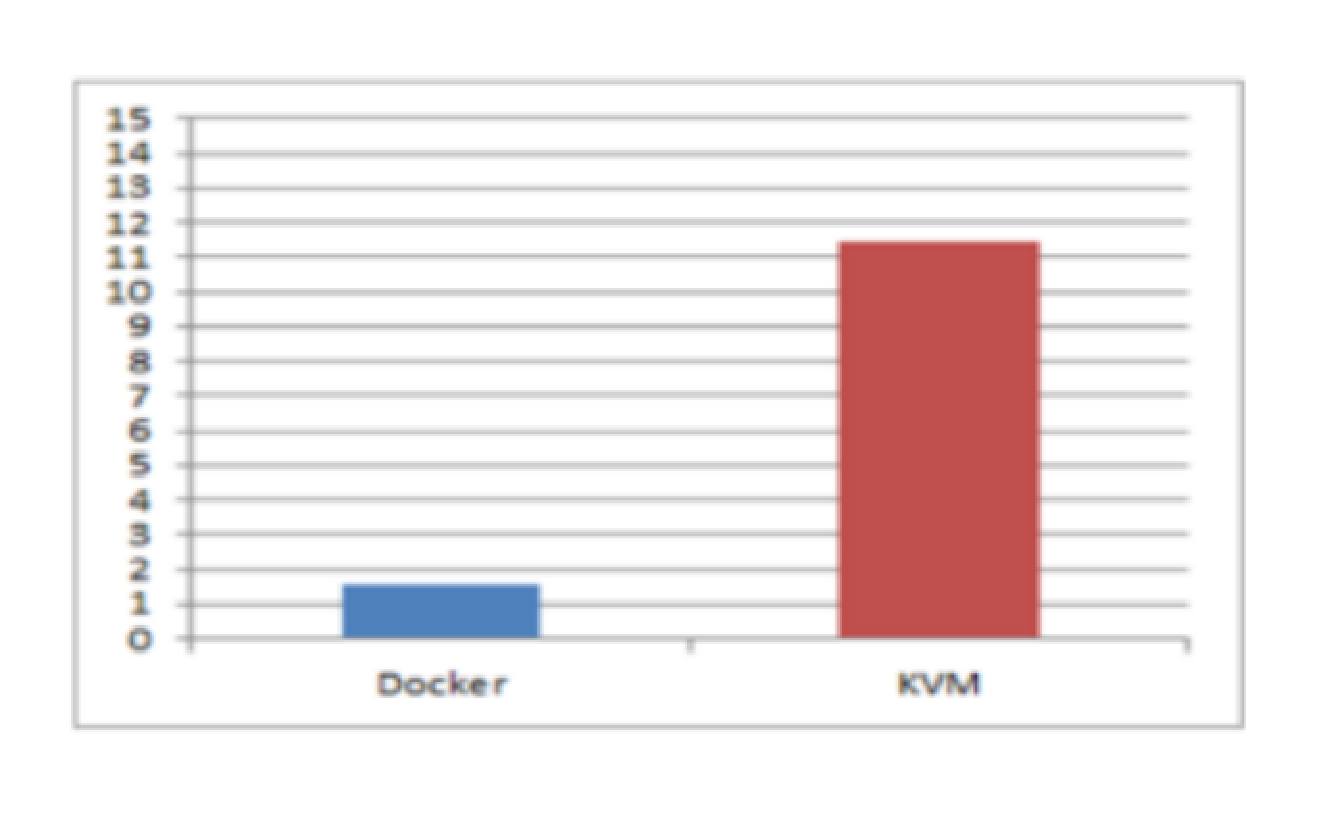
\psfig{file=docker_kvm.eps, height=2in, width=2in,}
\caption{Docker vs KVM Average boot time\cite{vdcp:seo}}
\label{fig:docker_kvm}
\vskip -6pt
\end{figure}

\subsection{Docker vs. KVM}

There are several comparisons between Virtual Machine and containerized technology. Seo et al\cite{vdcp:seo} used two servers with the same configurations in the cloud environment. One server runs the KVM\footnote{Kernel-based Virtual Machine (KVM) is a virtualization infrastructure for the Linux kernel that turns it into a hypervisor.}. The other one run the docker. Compared to Virtual Machine, as the Docker Cloud does not contain a guest operating system, Docker takes much less time in booting and calculations. In the figure \ref{fig:docker_kvm}, both the docker and KVM generated 20 images. Docker used 1.5 seconds while KVM used more than 11 seconds. 

\subsection{Xen vs. LXC}

Another comparison was XenServer6.2 with CoreOS 324.3.0 with Docker 0.11.1 on two identical machines. Their hardware environments are all the same. Scheepers (2014) \cite{vdcp:sche} used a PHP-script querying the database to test inter-virtual machine communication. The script was executed on a different virtual machine than the database. As figure \ref{fig:xen_core} shows, LXC takes less time because it experiences less overhead in networking and CPU utilization when querying the database. However, with another PHP-script which inserting randomly generated data into a database by utilizing all the available resources, the LXC take a lot of time more than the Xen. The reason is that of LXC's inability to successfully isolate resources. The result is shown in figure \ref{fig:xen_core2} 

\begin{figure}[htb]
\centering
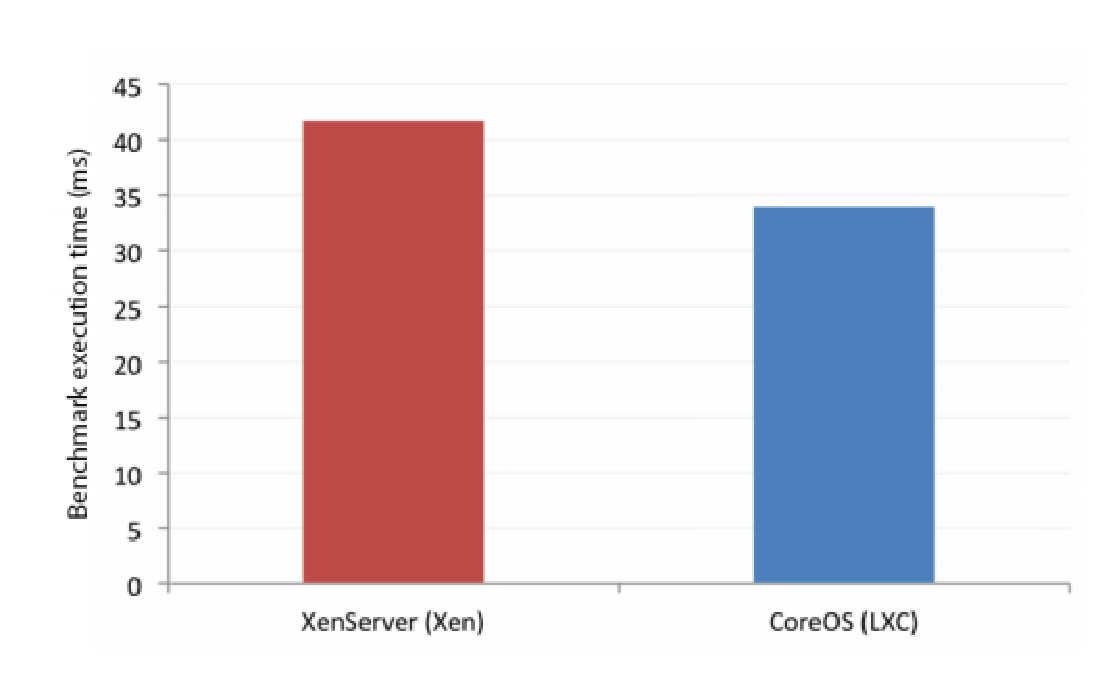
\psfig{file=Xen_Core.eps, height=2in, width=2in,}
\caption{Time in ms to complete one SQL SELECT query. (Less is better)\cite{vdcp:sche}}
\label{fig:xen_core}
\vskip -6pt
\end{figure}

\begin{figure}[htb]
\centering
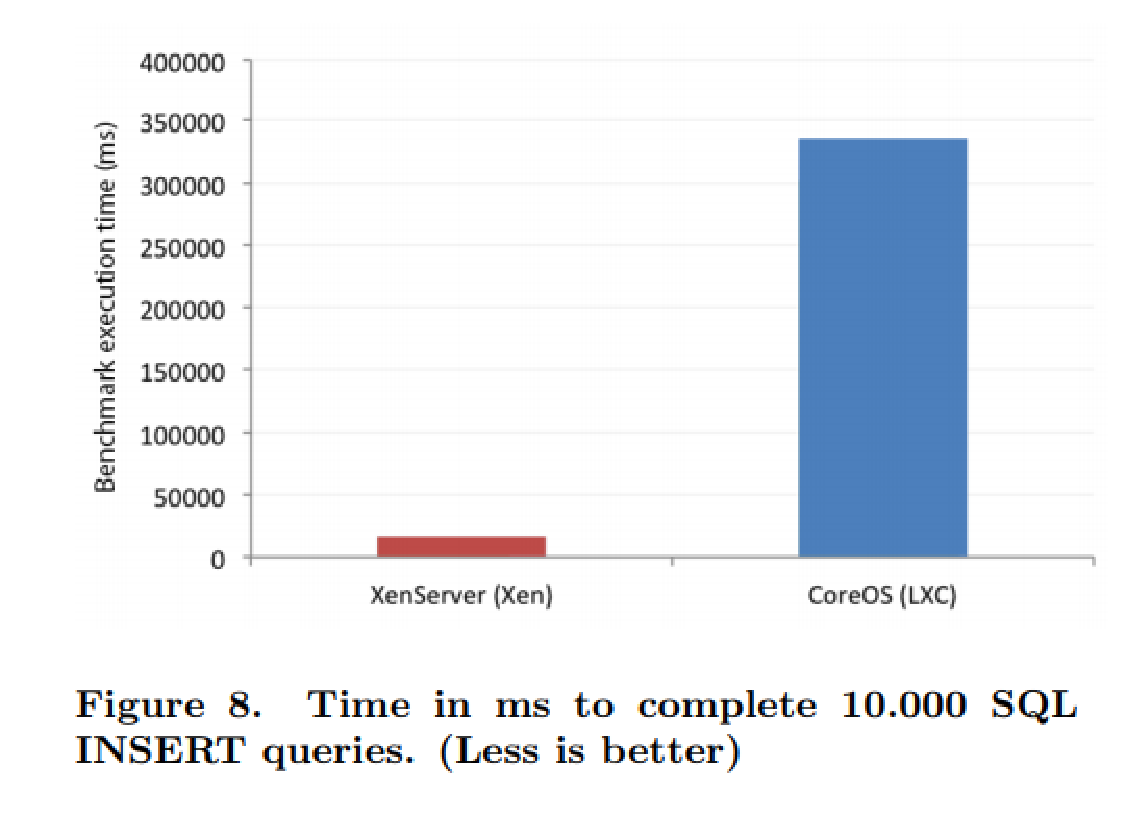
\psfig{file=Xen_Core2.eps, height=2in, width=2in,}
\caption{Time in ms to complete 10,000 SQL INSERT queries. (Less is better)\cite{vdcp:sche}}
\label{fig:xen_core2}
\vskip -6pt
\end{figure}

\begin{table*}[ht]
\label{tb:1}
\centering
    \begin{tabularx}{15cm}{|*{7}{C|}}
        \hline
        \multicolumn{2}{|c|}{\textbf{Seo et al. (2014)\cite{vdcp:seo}}} & \multicolumn{2}{|c|}{\textbf{Scheepers (2014) \cite{vdcp:sche}}} & \multicolumn{3}{|c|}{\textbf{Felter et al. (2014) \cite{vdcp:fel}}} \\
        \hline
        \textbf{Docker} & \textbf{KVM} & \textbf{XenServer (Xen)} & \textbf{CoreOS (LXC)} & \textbf{Native} & \textbf{Docker} & \textbf{KVM} \\
        \hline
            Boot Time short & Boot time long & Calculation Speed is faster & Calculation Speed is Slower & Overhead (wastage of resources) & Slightly less overhead than Native & Slightly less than Native and Docker \\
        \hline
        Calculation Speed is faster & Calculation Speed is Slower & Less time to accomplish request & Longer time to accomplish request & Slow Execution equal to Docker & Slow Execution equal to Native & Fast Execution \\
        \hline
        No Guest OS & Works Independently & Better in sense of equally distributing resources & Better in sense of executing isolated processes & - & Mature Innovation & Mature Innovation \\
        \hline
    \end{tabularx}
\caption{Comparison Table based on Different Virtual Machines and Containerized Technology}
\end{table*}

\subsection{I/O Native vs. Docker vs. KVM}
One more comparison we would like to mention is \textit{Block I/O}-fio.  We've already mentioned that virtualizing block storage could cause overhead. Felter (2014) \cite{vdcp:fel}  benchmarked the throughput of Native, Docker, and KVM in different scenarios. In figure \ref{fig:io_seq}, three have almost the same throughput which means the overhead in this scenario could be negligible. Things changed when the read and write became random (70\% read, 30 \% write). The Docker throughput stays the same as Native but the KVM drops half the throughput as figure \ref{fig:io_rd} shows. And more details are shown in figure \ref{fig:rd_read}, The Native and Docker lines are almost superimposed atop one another while KVM increases read latency by 2-3x, a crucial metric for some real workloads.

\begin{figure}[htb]
\centering
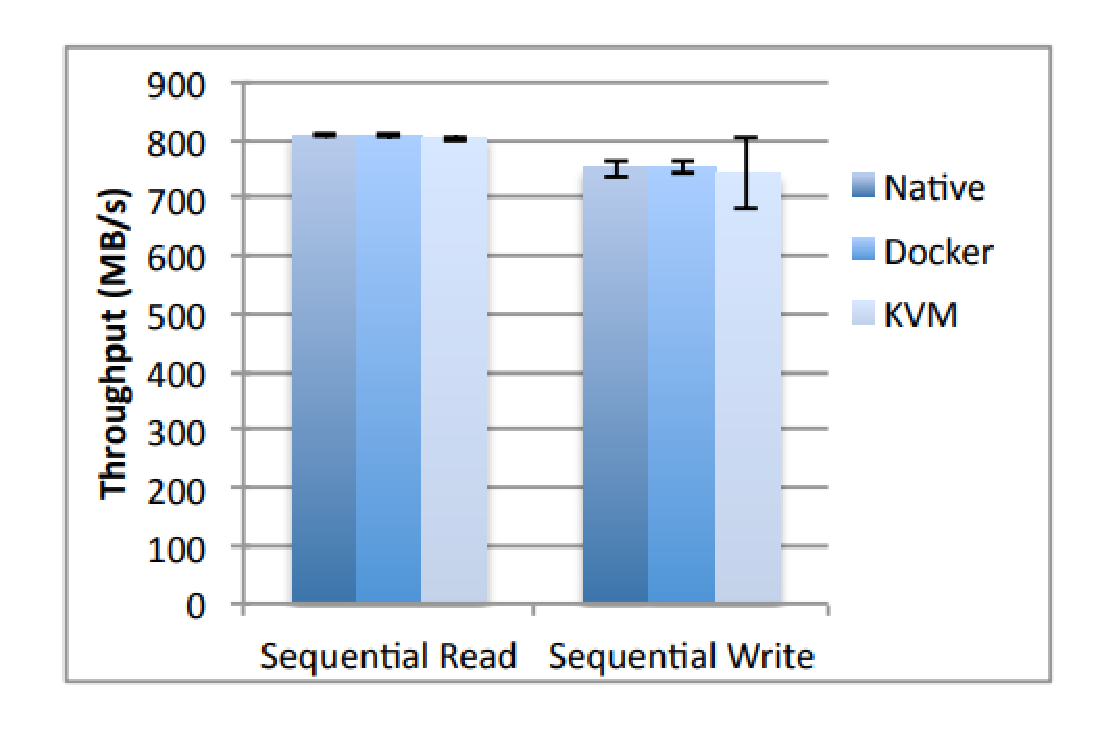
\psfig{file=IO_sequential.eps, height=2in, width=2in,}
\caption{Sequential I/O throughput (MB/s)\cite{vdcp:fel}}
\label{fig:io_seq}
\vskip -6pt
\end{figure}

\begin{figure}[htb]
\centering
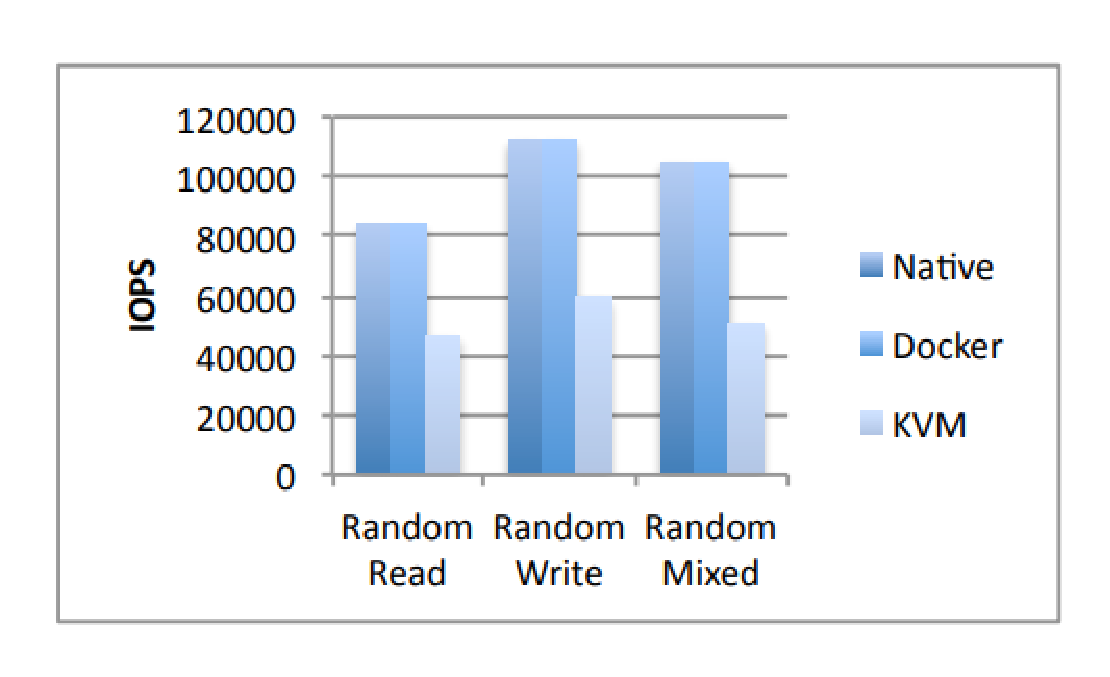
\psfig{file=IO_random.eps, height=2in, width=2in,}
\caption{Random I/O throughput (IOPS)\cite{vdcp:fel}}
\label{fig:io_rd}
\vskip -6pt
\end{figure}

\begin{figure}[htb]
\centering
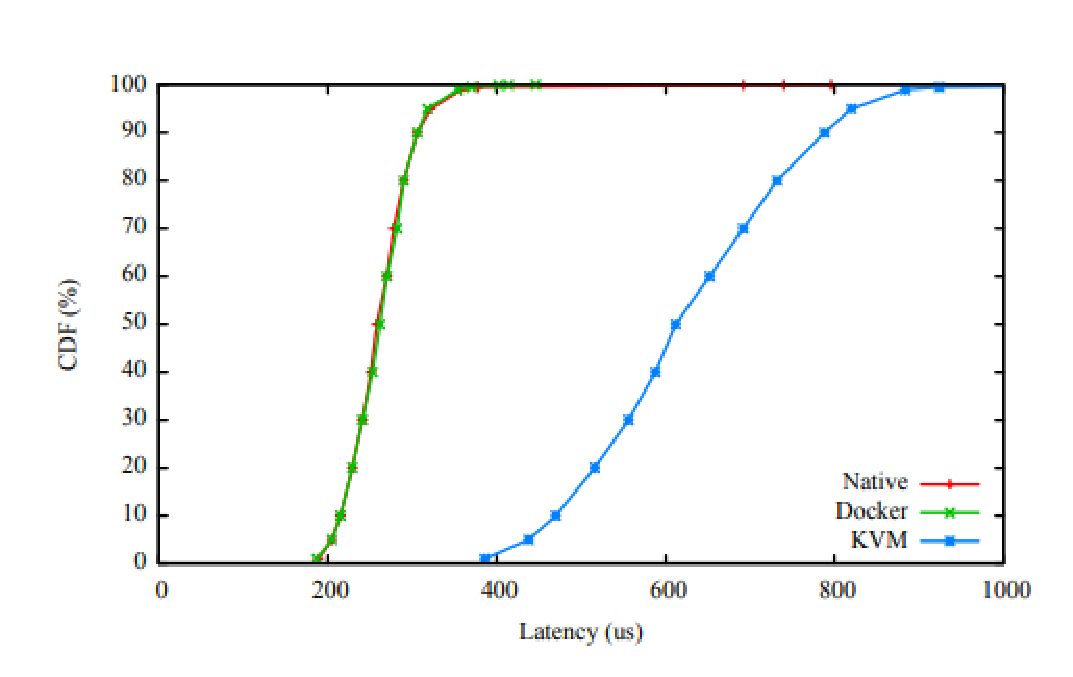
\psfig{file=Random_read.eps, height=2in, width=2in,}
\caption{Random read latency CDF, concurrency 16 ($\mu$ s). The Native and Docker lines are almost superimposed atop one another.\cite{vdcp:fel}}
\label{fig:rd_read}
\vskip -6pt
\end{figure}

\section{Short Summary}
Table \ref{tb:1} gives us an overview of comparisons between virtual machine and containerized technology. Docker, in most cases, has better performance as it avoids the overhead of running guest operating system and has less wastage of resource than VM.

\section{Conclusion}
Virtual Machine and Docker container are indeed very similar to each other, but they are not the same. Virtual Machine isolates the whole system while the docker container isolates applications. To decide which technology one should use, it still needs to depend on the requirement. Docker cannot total replace the virtual machine even it, in many cases, performs better than Virtual Machine. One big usage of Virtual Machine, as I mentioned at the beginning, is the cloud hosting. If you told your customers that you are using Docker containers and they will share the memory with other customers, they might not want to use your services. Another restriction is that you cannot have Windows docker running on a Linux kernel or vice versa. And, if your projection was to test the entire system, using docker would not be a good choice. All in all, if you were trying to isolate a single process, docker container would be much better.

\section{Acknowledgments} 
We'd like to thank Dr. Chen for his suggestions.
%
% The following two commands are all you need in the
% initial runs of your .tex file to
% produce the bibliography for the citations in your paper.
\bibliographystyle{abbrv}
\bibliography{main}  % sigproc.bib is the name of the Bibliography in this case
% You must have a proper ".bib" file
%  and remember to run:
% latex bibtex latex latex
% to resolve all references
%
% ACM needs 'a single self-contained file'!
%
%APPENDICES are optional
%\balancecolumns

\end{document}
